\documentclass[aspectratio=169, 11pt]{beamer}

% --- Packages & Setup ---
\usepackage[utf8]{inputenc}
\usepackage[T1]{fontenc}
\usepackage{xcolor}
\usepackage{booktabs}
\usepackage{graphicx}
\usepackage{tikz}
\usetikzlibrary{calc}

% Branding Colors
\definecolor{amritaMaroon}{HTML}{A4123F}

% Theme Setup
\usetheme{Madrid}
\usecolortheme[named=amritaMaroon]{structure}
\setbeamertemplate{navigation symbols}{}
\setbeamertemplate{footline}[frame number]

\begin{document}

% --- TITLE SLIDE ---
\begin{frame}
    \begin{tikzpicture}[remember picture,overlay]
        \node[fill=amritaMaroon, text=white, font=\bfseries\footnotesize, anchor=north east, rounded corners=2pt, inner sep=5pt]
        at ($(current page.north east) + (-0.2cm,-0.2cm)$)
        {Type 1: Research Project};
    \end{tikzpicture}

    \centering
    \vspace{0.2cm}
    
\includegraphics[width=2cm]{logo_square.png} % Local path
    \vspace{0.2cm}

    {\Large \textbf{\textcolor{amritaMaroon}{Explainable Federated Analytics for Multivariate Time-Series Forecasting with Personalized Model Adaptation}}} \\
    \vspace{0.1cm}
    {\small \textbf{Team Number: 28 | Review 2 (Technical Progress)}} \\
    \vspace{0.2cm}

    \begin{table}
        \centering
        \footnotesize
        \renewcommand{\arraystretch}{0.9}
        \begin{tabular}{|c|c|l|}
            \hline
            \textbf{S.No} & \textbf{Register Number} & \textbf{Student Name} \\
            \hline
            1 & CB.SC.U4CSE23363 & Haswitha K \\
            \hline
            2 & CB.SC.U4CSE23529 & Hasini Reddy M \\
            \hline
            3 & CB.SC.U4CSE23547 & Sheela Akshar Sakhi \\
            \hline
            4 & CB.SC.U4CSE23761 & Kousik Sarma Lakkaraju \\
            \hline
            5 & CB.SC.U4CSE23753 & V.Chakravarthy \\
            \hline
        \end{tabular}
    \end{table}

    {\footnotesize
    Guide: \textbf{Dr. G R RAMYA, Dr. VANDHANA S} \\
    Department of CSE
    }
\end{frame}

% --- PANEL COMMENTS RESPONSE ---
\begin{frame}{Addressing Panel Review 1 Comments}
    \small
    \begin{itemize}
        \item \textbf{Scope \& Use Case:} Narrowed to \textbf{Smart Energy Grid Load Forecasting}.
        \item \textbf{Research Novelty:} Explicit role of \textbf{CUSUM Drift Detection} established.
        \item \textbf{Technical Depth:} Internal mechanics of \textbf{CUSUM} and \textbf{Attention} elucidated.
        \item \textbf{Privacy:} Distinguished between \textbf{General Privacy} (No raw data) and \textbf{Differential Privacy} ($\epsilon$-DP noise).
        \item \textbf{Comparison:} Comparative study between \textbf{FedAvg}, \textbf{FedPer},and \textbf{FedProp} included.
    \end{itemize}
\end{frame}

% --- LITERATURE SURVEY SUMMARY ---
\begin{frame}{Literature Foundation (25 Papers)}
    \small
    \begin{columns}
        \begin{column}{0.6\textwidth}
            \textbf{Key Clusters Analyzed:}
            \begin{itemize}
                \item \textbf{FL Basics:} FedAvg (McMahan 2017) $\rightarrow$ Foundation.
                \item \textbf{Personalization:} FedPer (Arivazhagan 2020) $\rightarrow$ Heterogeneity handling.
                \item \textbf{Drift Detection:} CDA-FedAvg (Jothimurugesan 2022) $\rightarrow$ Adaptation.
                \item \textbf{Explainability:} Attention-LSTM (La Rocca 2021) $\rightarrow$ XAI.
            \end{itemize}
            \vspace{0.2cm}
            \begin{block}{The Research Gap}
            No existing framework simultaneously integrates \textbf{Personalization + Active Drift Monitoring + Explainable Attention} for Multivariate Time-Series.
            \end{block}
        \end{column}
        \begin{column}{0.4\textwidth}
            \centering
            
\includegraphics[width=0.8\linewidth]{logo_square.png}
            \vspace{0.2cm}
            \tiny \\ \textit{Full survey of 25 papers available in Review 1 documentation and Repository.}
        \end{column}
    \end{columns}
\end{frame}

% --- TARGETED PROBLEM STATEMENT ---
\section{Problem Statement}
\begin{frame}{Targeted Problem Statement: Smart Grids}
    \begin{block}{The Challenge}
        Accurate Household Load Forecasting (STLF) is hindered by:
        \begin{itemize}
            \item \textbf{Data Privacy:} Smart meter data is sensitive and regulated.
            \item \textbf{High Heterogeneity:} Diverse life styles (EV chargers vs. low-usage homes).
            \item \textbf{Concept Drift:} Demand shifts due to seasonality and behavior.
        \end{itemize}
    \end{block}

    \vspace{0.2cm}
    \textbf{Objective:} Develop a Federated Personalized Drift-Aware Attention Framework (\textbf{FPDAF}) specifically for Smart Grid analytics that maintains local privacy while adapting to individual house behavior and shifting demand.
\end{frame}

% --- SYSTEM ARCHITECTURE ---
\begin{frame}{System Architecture}
    \centering
    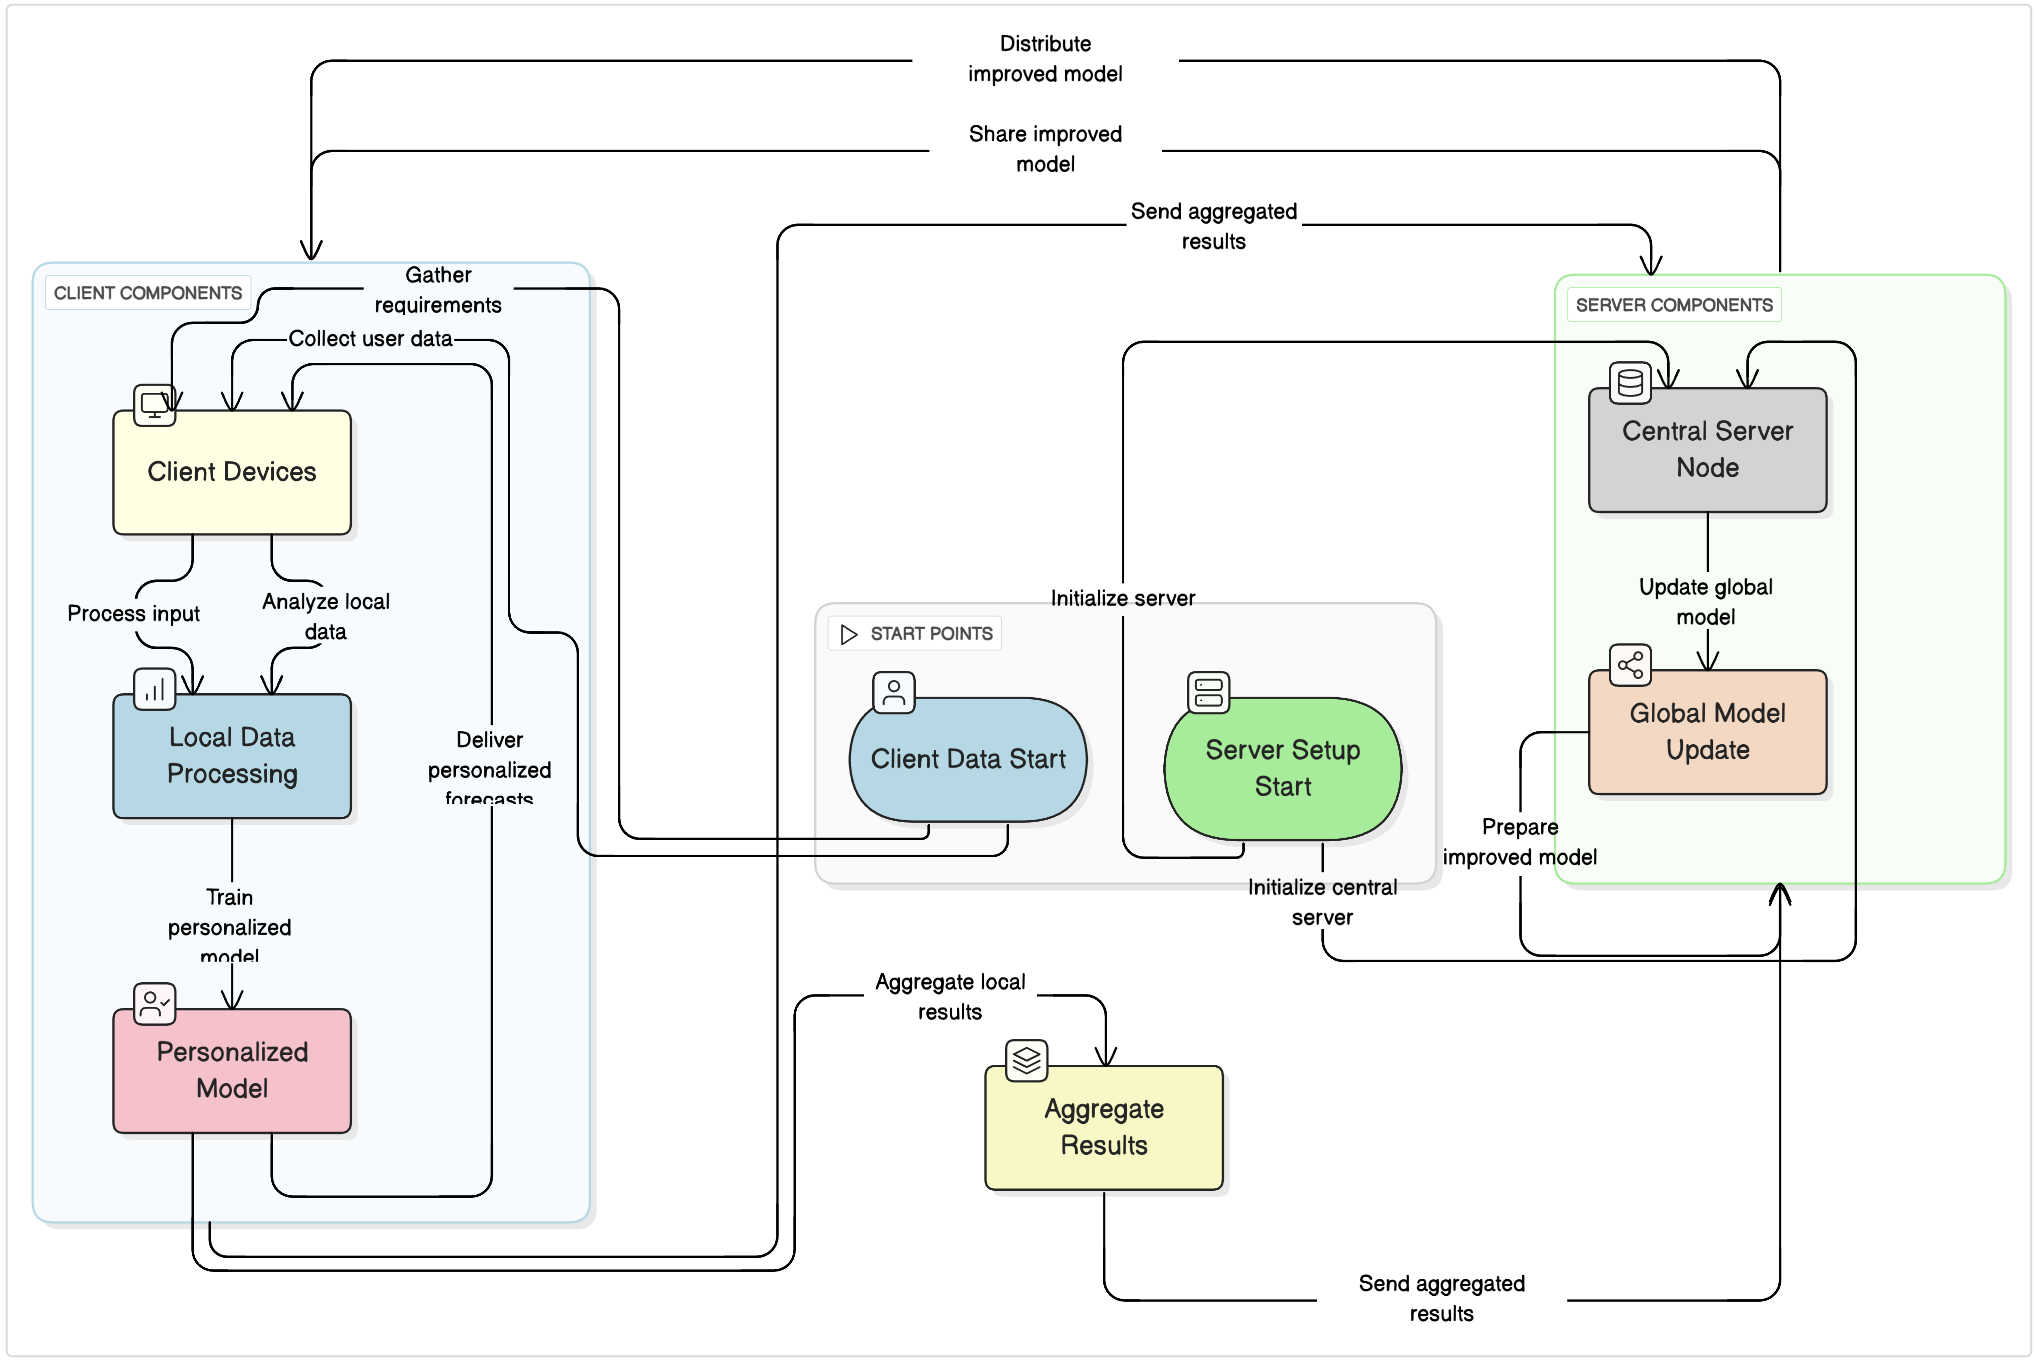
\includegraphics[width=0.8\linewidth, height=0.75\textheight, keepaspectratio]{SA_1.png}
    \caption{\small Hybrid Global-Personalized Federated Architecture with Attention}
\end{frame}

% --- NOVELTY & DRIFT HANDLING ---
\section{Technical Depth}
\begin{frame}{Technical Workflow: Drift Adaptation}
    \begin{columns}
        \begin{column}{0.5\textwidth}
            \textbf{CUSUM Trigger Mechanism:}
            \[ S_t = \max(0, S_{t-1} + (e_t - \mu - k)) \]
            \begin{itemize}
                \item \textbf{Phase 1:} Local loss residual monitoring.
                \item \textbf{Phase 2:} Threshold $h$ violation detection.
                \item \textbf{Phase 3:} On-demand local head retraining.
                \item \textbf{Phase 4:} Communication-efficient sync.
            \end{itemize}
        \end{column}
        \begin{column}{0.5\textwidth}
            \centering
            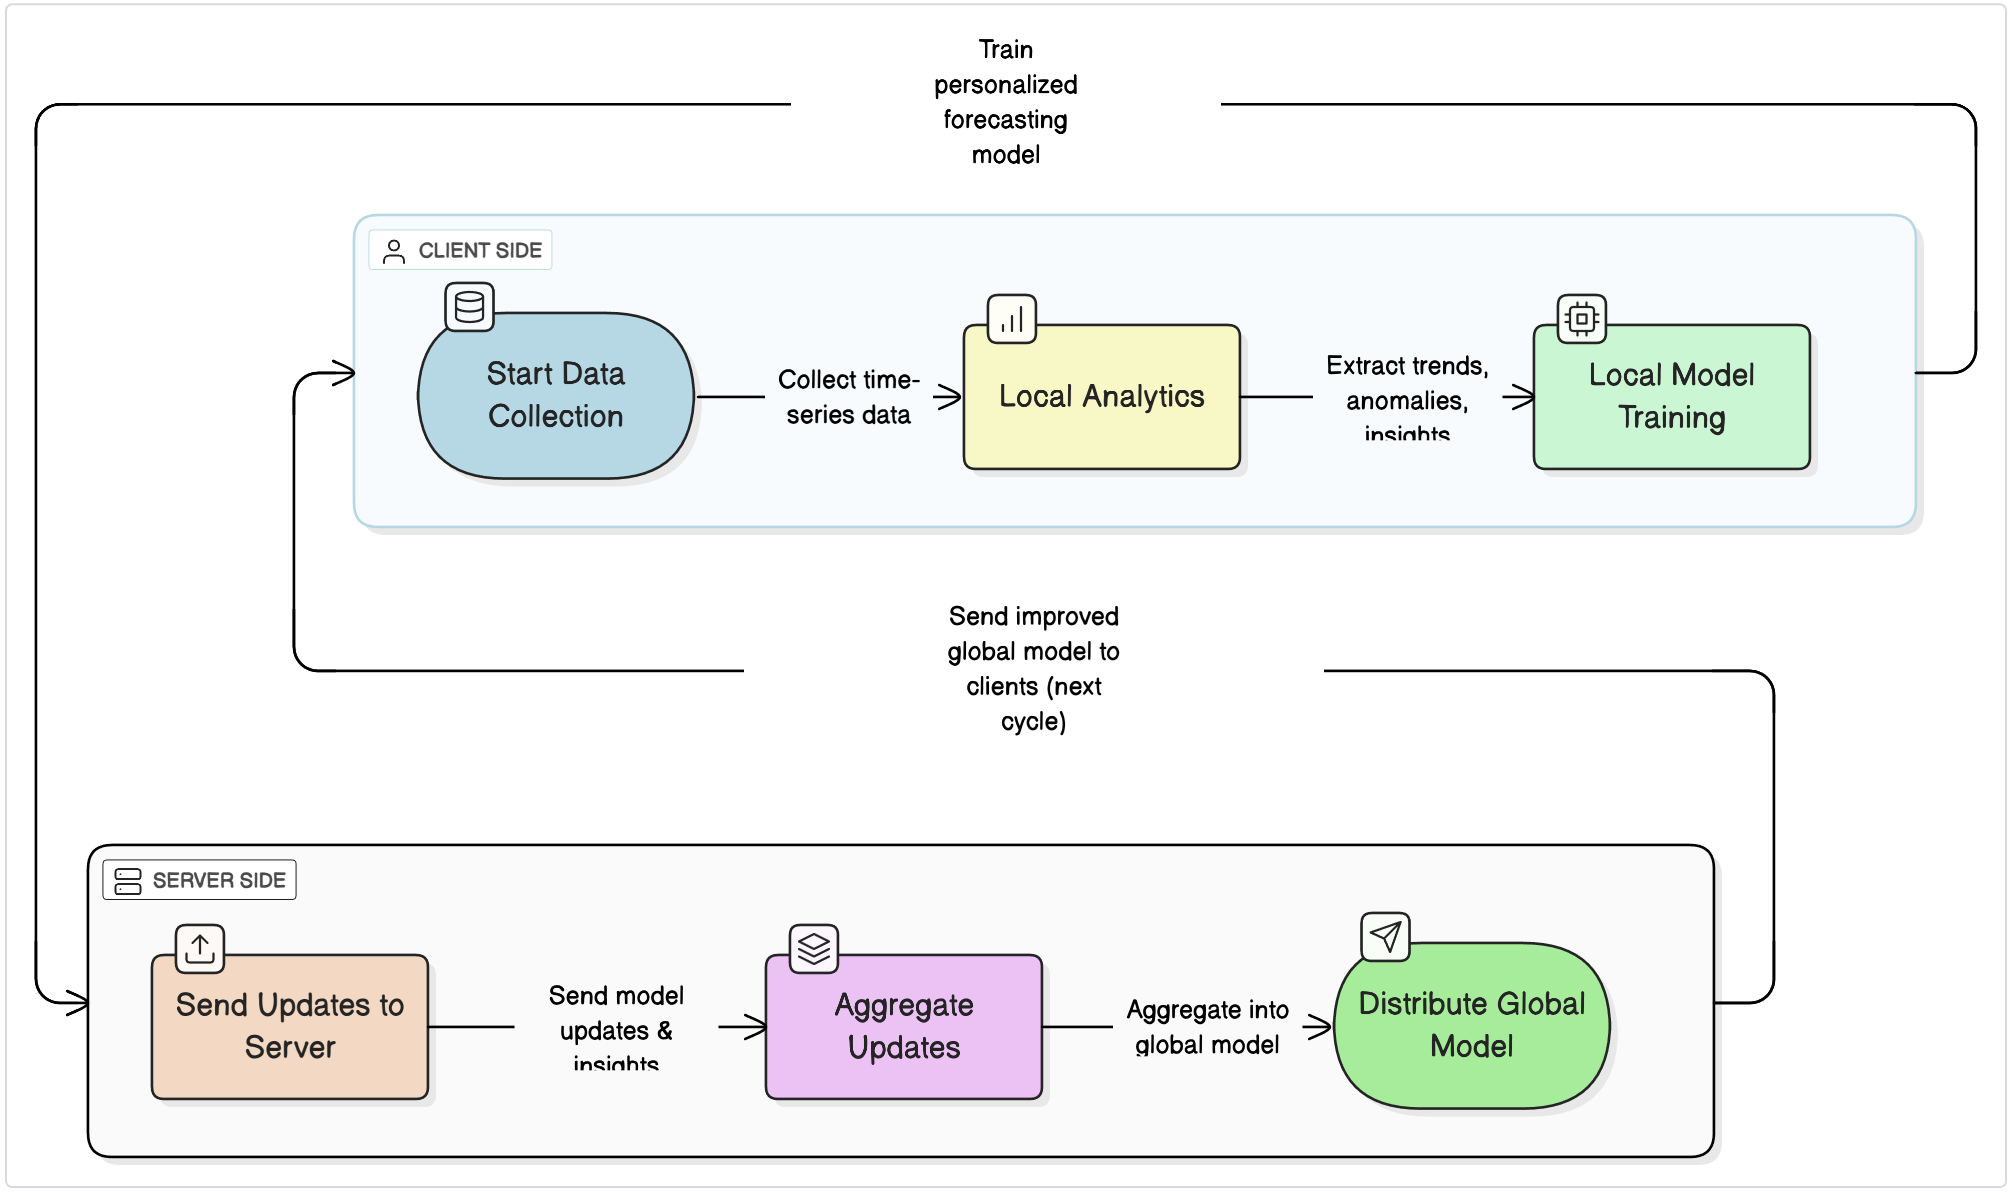
\includegraphics[width=1\linewidth]{AWF.png}
        \end{column}
    \end{columns}
\end{frame}

% --- TECHNICAL OVERVIEW ---
\begin{frame}{Internal Mechanics: Components}
    \begin{columns}
        \begin{column}{0.5\textwidth}
            \begin{block}{Personalized Model Head}
                \small Mapping shared patterns to house-specific habits via local MLP layers. Handles \textbf{Non-IID} data.
            \end{block}
            \begin{block}{Temporal Attention}
                \small Weighs historical timesteps based on importance. Explains \textit{when} the demand spike originated.
            \end{block}
        \end{column}
        \begin{column}{0.5\textwidth}
            \begin{block}{Differential Privacy ($\epsilon$-DP)}
                \small Adding Laplacian noise to model updates. Ensures formal mathematical guarantee against model inversion.
            \end{block}
            \begin{block}{Weighted Aggregation}
                \small Communication-efficient merge of local updates based on data volume ($n_i/n$).
            \end{block}
        \end{column}
    \end{columns}
\end{frame}

% --- COMPARATIVE STUDY ---
\section{Evaluation}
\begin{frame}{Comparative Discussion of Federated Methods}
    \centering
    \small
    \begin{table}
        \begin{tabular}{l p{2.5cm} p{2cm} p{2.5cm}}
            \toprule
            \textbf{Method} & \textbf{Handling Heterogeneity} & \textbf{Explainability} & \textbf{Drift Handling} \\
            \midrule
            FedAvg & Poor (one-size-fits-all) & No & None \\
            FedPer & Good (Local heads) & No & None \\
            FedProp & Good (Regularization) & No & Static \\
            \midrule
            \textbf{FPDAF} & \textbf{Optimal (Personal)} & \textbf{Yes (Attention)} & \textbf{Active (CUSUM)} \\
            \bottomrule
        \end{tabular}
    \end{table}
    \vspace{0.3cm}
    \textbf{Choice Justification:} Only FPDAF addresses the triad of \textit{Privacy, Adaptability, and Interpretability} required for trustworthy grid management.
\end{frame}

% --- STATUS & REPOSITORY ---
\section{Progress}
\begin{frame}{Current Status \& Evidence}
    \begin{itemize}
        \item \textbf{Git Repository:} Active version control with 20+ commits and structured reviews.
        \item \textbf{Technical Proof:} Mathematical simulation of CUSUM-FL completed.
        \item \textbf{Baseline Results:} Initial FedAvg benchmarks on Pecan Street dataset.
        \item \textbf{Future Plan:} Integration of $\epsilon$-Differential Privacy noise layers.
    \end{itemize}
    \centering
    \vspace{0.3cm}
    \textbf{Repo:} [github.com/aksharsakhi/23CSE399-Project-Phase-1]
\end{frame}

% --- REFERENCES ---
\begin{frame}[allowframebreaks]{Selected References}
    \tiny
    \nocite{mcmahan2017,arivazhagan2020,jothimurugesan2022,larocca2021attention,kalakoti2025fedxai}
    \bibliographystyle{IEEEtran}
    \bibliography{ref}
\end{frame}

% --- THANK YOU ---
\begin{frame}
    \centering
    {\Huge \textbf{\textcolor{amritaMaroon}{Thank You}}}
    \vspace{1cm}
    {\large Questions?}
\end{frame}

\end{document}
